\section{Discussion}

\subsection{Poor Performance of Recommended Parameters}

We had hypothesized that the strange beam shape and low sample current were caused by the filament being too hot. With the cathode voltage being at 
its maximum value, this was most likely placing the beam in a space charge limited configuration. One can see that the maximum observed current in 
figure \ref{fig:badbeam} was just $0.4\mu$A, which is an entire order of magnitude lower than the maximum current observed in the optimized beam. 
This has all of the characteristics of a space charge limited beam, meaning that the high temperature was indeed why we were not getting a well 
behaved beam. 

Explaining the observed shape is slightly more challenging. Stoffel and Johnson\cite{stoffel1985low} provide a figure (fig. \ref{fig:cath}) in their work outlining their gun design
that examines how cathode temperature affects beam emission. At a low temperature electrons emitted from the cathode's surface and passing through 
an aperture form a diverging beam with a single apparent source within the cathode. At an increased temperature, the thermal energy distribution is 
broadened and so the resulting beam appears to come from multiple source points withing the cathode. Our space charge limited beam can be described by 
the second case. The beam is broader than that of the low temperature cathode, and there are multiple points of overlap from the apparent sources. It 
is possible that the regions of overlap, after going through the electron optics, were focused to the beam's edge. This would explain both why there 
was a higher current at the edge, and why the electrons located there were at a lower energy then the electrons at the centre. 

\begin{figure}[h!]
    \centering
    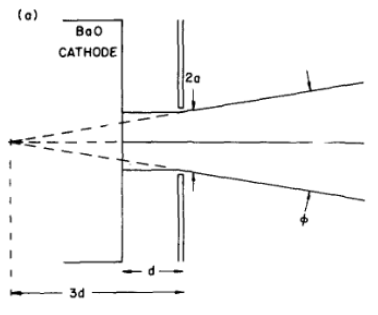
\includegraphics[width=0.45\linewidth]{../Assets/Low Temp.png}
    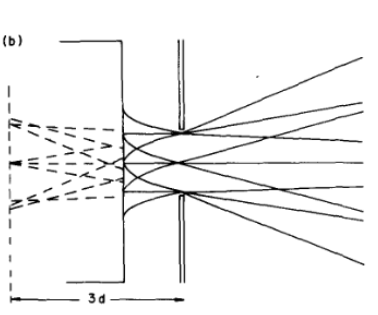
\includegraphics[width=0.45\linewidth]{../Assets/High Temp.png}
    \caption{Left: Emission from cathode operating in temperature limited mode. The dotted line indicate the apparent point source of the electron 
    beam, located within the cathode. Right: Emission from high temperature, space charge limited cathode. The widened beam now appears to come 
    from multiple apparent point sources\cite{stoffel1985low}}
    \label{fig:cath}
\end{figure}

\subsection{Optimized Beam Performance}

Our beam has a minimum FWHM of $2.148\pm0.013$mm, though as is stated in \cite{raj2004optimization} this is not truly indicative of the beam's spot size. 
Instead this represents a convolution of the beam's true gaussian profile with a rectangular function which reflects the aperture of the Faraday cup.
To find the true width of the beam, we convolve a boxcar function with a 1mm width (the size of the Faraday cup opening), with a general gaussian function. 
By then performing a non-linear fit of this convolution function to the minimum beam width data we are able to find a more representative FWHM for 
our beam, see figure \ref{fig:convolution}. We obtained a result of $2.033\pm0.014$mm, smaller than obtained from the raw data and in strong agreement with the results obtained by other 
groups\cite{raj2004optimization,ipes,Ciccacci}. These groups also report divergence angles in the range of $3^\circ$ to $7^\circ$, which our value 
of $4.15\pm0.50^\circ$ falls on the low end of. All of these groups have managed to publish novel and high quality results, indicating a strong 
future for our spectrometer once final characterization is complete.

\begin{figure}[h!]
    \centering
    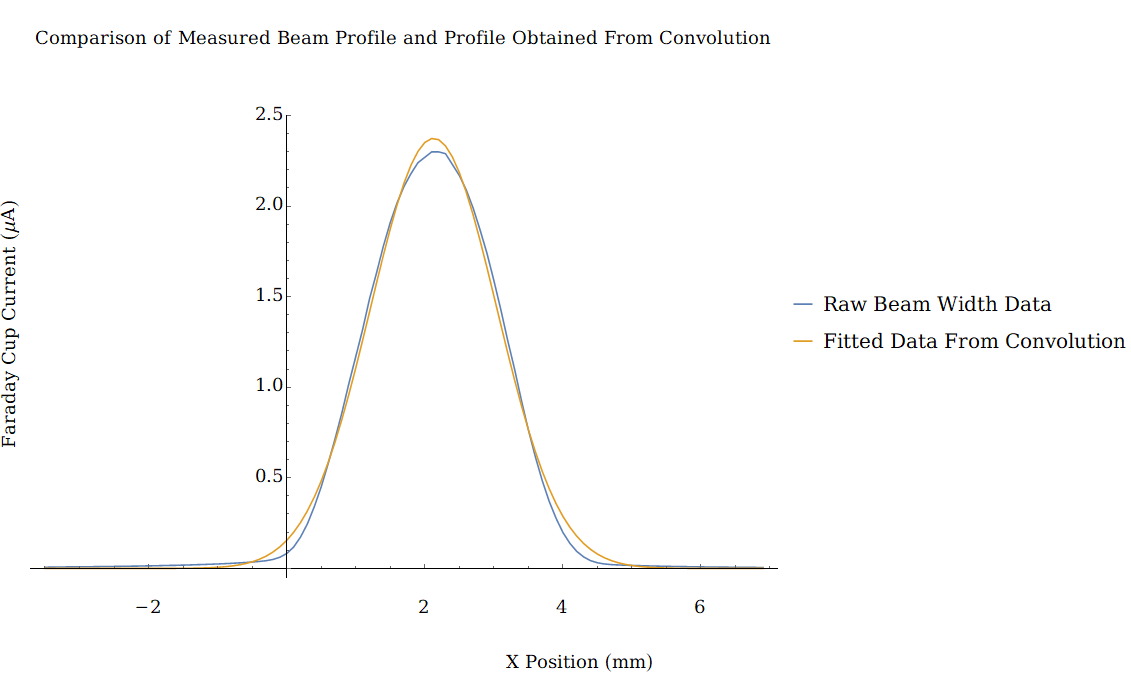
\includegraphics[width=0.85\linewidth]{../Beam Divergence/Plots/Convolution.png}
    \caption{Comparison of raw beam width data to the curve produced by convoluting a 1mm boxcar with a general gaussian function, and performing 
    a non-linear best fit.}
    \label{fig:convolution}
\end{figure}

We were able to use the divergence angle to calculate a momentum resolution of our beam, which we found to be $(1.07\pm0.13)\times10^9\mathrm{m}^{-1}$. 
If a beam's momentum resolution is too large, we will be unable to resolve fine details in the electronic structure of samples we are studying. 
A good way to put the value for $\Delta k_\parallel$ into context is to compare it to the size of the first brillouin zone of copper. Copper has 
an FCC unit cell, with a lattice constant, $a$, of 361.49pm\cite{reference.wolfram_2021_elementdata}. The size of the brillouin zone is given by:
\begin{equation}
    d = \frac{2\pi}{a}
\end{equation}
from which we find that the brillouin zone's size is  $1.74\times10^{10}\mathrm{m}^{-1}$. This is a full order of magnitude larger than our beam's momentum 
resolution, implying that our beam is fully capable of resolving features within copper's first brillouin zone. 

Our optimized electron gun configuration meets every requirement of inverse photoemission, aligns strongly with the results of groups with 
comparable setups, and is capable of resolving features in the copper brillouin zone. We feel that we have successfully characterized the gun to the 
extent that it is capable of producing quality spectra, and any further improvements will most likely be marginal. 

\subsection{Failure of KRIPES Experiment}

While it is true that our gun should be able to resolve features in the first brillouin zone of copper, our angle resolved IPES experiments showed 
no agreement with what was published by Budke et al. In fact, the spectra obtained showed hardly any of the expected features of a typical IPES 
spectrum, with the results of $\theta=0^\circ$ only marginally meeting expectations. The previous section has demonstrated that our electron gun 
is more than capable of being used for inverse photoemission, and the photodetectors were characterized in Phys 437A meaning that our system should 
be able to produce an IPES spectrum for Cu(111). The only other main contributing factor is the quality of the sample's surface. As was discussed in 
the sample preparation section, our copper sample was left in a high vacuum environment once Phys 437A was completed, for a total time of roughly 
three months before the KRIPES experiment was performed.

The only mechanism by which a sample in high vacuum can degrade is through chemical reaction with, or adsorption of the residual gas in the chamber.
A previous member of our group\cite{mcmahon_2012,lafferty_1998} determined that the completed fraction of the first monolayer formed after an elapsed time $F(t)$
for a sample with sticking coefficient $\alpha$, and total number of binding sites $\eta$ is given by:

\begin{equation}
    F(t) = \frac{\alpha P}{\eta \sqrt{2\pi m kT}}t
\end{equation}

For a worst case estimate of our copper sample, we assume that $\alpha=1$ meaning every gas particle that hits the sample will be adsorbed. We can 
then approximate the value of $\eta$ using the properties of copper\cite{mcmahon_2012}; specifically its atomic weight of approximately 64g/mol, 
and a density of approximately 9g/cm$^3$. Finally, an assumption of 1 binding site per copper atom, and simplifying its crystal structure to a 
simple cubic lattice we obtain $\eta\approx1\times10^{15}$. 

Hydrogen gas has the highest concentration in ultra high vacuum systems due to outgassing from the stainless steel chamber\cite{article}, and is also
difficult for cryopumps and turbomolecular pumps to remove from the system\cite{danielson}. Assuming that all of the incident gas particles 
are H$_2$ then we finally obtain that the time for a single monolayer to form at a pressure $P$ is given by:

\begin{equation}
    t\approx\frac{1.35\times10^{-6}[\mathrm{torr\cdot s}]}{P}
\end{equation}

With the maximum pressure our sample was exposed to being roughly $9\times10^{-10}$ torr, then a single monolayer in the worst case forms on the sample
in 1500s, or 25 minutes. This is certainly much faster than a monolayer of adsorbed H$_2$ would form on our Cu sample, but even if it formed one thousand 
times slower the surface would only be clean for 17 days. Depending on monolayer thickness, multiple layers may need to be formed before electrons are 
prevented from reaching the sample's bulk. However with the sample being in the vacuum environment for roughly 90 days prior to the IPES measurements it is clear 
that it had degraded too much for us to be able to observe a surface sensitive feature. 

To verify this we would simply need to re-clean the surface of the sample using Argon ion etching and annealing and run an IPES scan immediately 
after the sample has cooled. Sadly our sample was damaged during a transfer so we were unable to do so, but this provides us with a starting point 
when a new sample is acquired. 

\section{Conclusions}

We sought to characterize the performance of our spectrometer's low energy electron gun. The manufacturer recommended parameters were used 
as a starting point, and they produced a beam which was not fit for inverse photoemission applications. The beam was several times larger than 
desired, and had a poorly collimated profile. By examining the electron energy distributions at specific locations in the beam and reducing the 
temperature of the cathode we determined that the beam was heavily space charge limited under these conditions. A broad search of parameter space
at this reduced temperature yielded a configuration which met all of the requirements for inverse photoemission. 

The successful characterization of our electron gun marks the end of our major characterization work needed for inverse photoemission spectroscopy. 
Our gun was found to produce a beam with a minimum width of 2.033mm, with a 4.15$^\circ$ divergence angle. This is comparable to the results
reported by many groups who have already published novel IPES studies. With a momentum resolution of $1.07\times10^9\mathrm{m}^{-1}$, an order of 
magnitude smaller than the first brillouin zone of copper, we expect that our spectrometer will soon be producing results which align very closely 
to the numerous IPES benchmarks in the literature. 

Future work on this project will involve improvements to our vacuum environment to prolong sample lifetime, procuring and preparing another Cu(111) sample, and attempting to replicate the results published in IPES studies.

\clearpage

\section{Acknowledgments}

My time in Phys 437 has been one of the most informative experiences of my undergrad. The requirements to be an experimentalist are, lacking a better word,
overwhelming. However, thanks to my supervisor David Hawthorn I felt ready to tackle any challenge we faced in the lab. He is always there to answer
any questions I may have, and provide suggestions on where our work should head next. I've learned a great deal during my time working in his lab, 
about both the areas of physics I'm most passionate about, and on how to perform quality physics research. Thankfully my time with the group is not 
over, and I'll be continuing to work on this project in the coming months. I'm greatly looking forward to the opportunity.

To my fellow students in the Hawthorn group, specifically Yuxuan Qi and Naman Gupta, I thank you for your insight and many conversations trying to fix 
our spectrometer's issues. It always feels better when I'm not the only one baffled by it. 

Finally, thank you to the readers of this report who dedicate your time to provide feedback for students such as myself who are developing our research skills.
